\documentclass[border=12pt]{standalone}
\usepackage{tikz}
\usetikzlibrary{positioning,shapes,arrows.meta}

\begin{document}
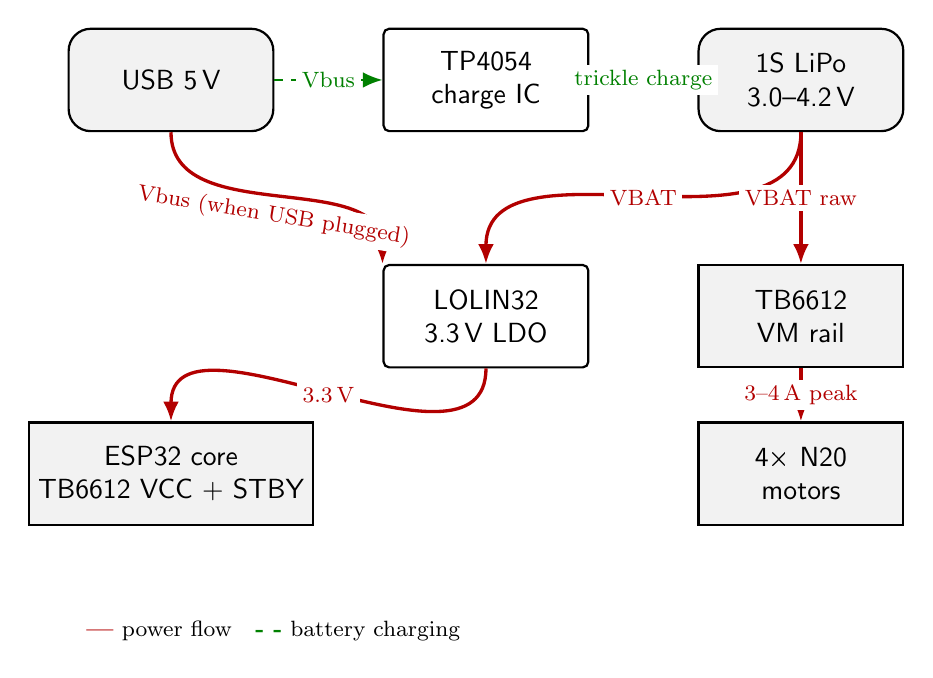
\begin{tikzpicture}[
  font=\sffamily,
  block/.style={
    draw, thick, rounded corners=2pt,
    minimum width=2.6cm, minimum height=1.3cm,
    align=center, fill=white,
  },
  source/.style={
    draw, thick, rounded corners=8pt,
    minimum width=2.6cm, minimum height=1.3cm,
    align=center, fill=black!5,
  },
  load/.style={
    draw, thick, rectangle,
    minimum width=2.6cm, minimum height=1.3cm,
    align=center, fill=black!5,
  },
  pwr/.style={-{Latex[length=2.5mm,width=2mm]}, very thick, color=red!70!black},
  charge/.style={-{Latex[length=2.5mm,width=2mm]}, thick, color=green!50!black, dashed},
  ann/.style={font=\footnotesize, fill=white, inner sep=2pt},
]

\node[source] (usb) at (0,3) {USB 5\,V};
\node[block] (tp) at (4,3) {TP4054\\charge IC};
\node[source] (bat) at (8,3) {1S LiPo\\3.0–4.2\,V};

\node[block] (ldo) at (4,0) {LOLIN32\\3.3\,V LDO};
\node[load] (logic) at (0,-2) {ESP32 core\\TB6612 VCC + STBY};
\node[load] (vm) at (8,0) {TB6612\\VM rail};
\node[load] (mot) at (8,-2) {4× N20\\motors};

\draw[charge] (usb.east) -- node[ann]{Vbus} (tp.west);
\draw[charge] (tp.east) -- node[ann]{trickle charge} (bat.west);
\draw[pwr] (usb.south) to[out=-90,in=90] node[ann,sloped,below]{Vbus (when USB plugged)} (ldo.north west);
\draw[pwr] (bat.south) to[out=-90,in=90] node[ann]{VBAT} (ldo.north);
\draw[pwr] (bat.south) to[out=-90,in=90] node[ann]{VBAT raw} (vm.north);
\draw[pwr] (ldo.south) to[out=-90,in=90] node[ann]{3.3\,V} (logic.north);
\draw[pwr] (vm.south) -- node[ann]{3–4\,A peak} (mot.north);

\node[font=\footnotesize, anchor=west] at (-1.2,-4) {%
  \textcolor{red!70!black}{\textbf{---}} power flow\quad
  \textcolor{green!50!black}{\textbf{- -}} battery charging
};

\end{tikzpicture}
\end{document}
